\documentclass[12pt,a4paper]{report}

% Modern packages for professional formatting
\usepackage[utf8]{inputenc}
\usepackage[T1]{fontenc}
\usepackage[english,french]{babel}
\usepackage[margin=2.5cm]{geometry}
\usepackage{graphicx}
\usepackage{xcolor}
\usepackage{hyperref}
\usepackage{titlesec}
\usepackage{fancyhdr}
\usepackage{tocloft}
\usepackage{afterpage}
\usepackage{pdfpages}
\usepackage{float}
\usepackage{caption}
\usepackage{subcaption}
\usepackage{enumitem}
\usepackage{array}
\usepackage{booktabs}
\usepackage{longtable}
\usepackage{setspace}
\usepackage{parskip}

% Color definitions
\definecolor{espritblue}{RGB}{0,48,135}
\definecolor{imtgray}{RGB}{102,102,102}
\definecolor{sectioncolor}{RGB}{0,48,135}

% Hyperref setup
\hypersetup{
    colorlinks=true,
    linkcolor=espritblue,
    filecolor=magenta,
    urlcolor=espritblue,
    citecolor=espritblue,
    pdftitle={Dossier de candidature - Mobilité bi-diplômante IMT Mines Albi},
    pdfauthor={Fedi HMIDA},
    pdfsubject={Candidature Double Diplôme},
    pdfkeywords={IMT Mines Albi, Double Diplôme, Esprit, Mobilité étudiante, Fedi Hmida}
}

% Title formatting
\titleformat{\chapter}[display]
{\normalfont\huge\bfseries\color{sectioncolor}}
{\chaptertitlename\ \thechapter}{20pt}{\Huge}

\titleformat{\section}
{\normalfont\Large\bfseries\color{sectioncolor}}
{\thesection}{1em}{}

\titleformat{\subsection}
{\normalfont\large\bfseries\color{sectioncolor}}
{\thesubsection}{1em}{}

% Header and footer setup
\pagestyle{fancy}
\fancyhf{}
\fancyhead[L]{\textcolor{espritblue}{\textbf{Fedi HMIDA - Dossier de candidature IMT Mines Albi}}}
\fancyhead[R]{\textcolor{imtgray}{\thepage}}
\fancyfoot[C]{\textcolor{imtgray}{\small Esprit - École d'Ingénieurs}}
\renewcommand{\headrulewidth}{0.5pt}
\renewcommand{\footrulewidth}{0.3pt}
\renewcommand{\headrule}{\hbox to\headwidth{\color{espritblue}\leaders\hrule height \headrulewidth\hfill}}
\renewcommand{\footrule}{\hbox to\headwidth{\color{imtgray}\leaders\hrule height \footrulewidth\hfill}}

% Table of contents formatting
\renewcommand{\cftchapfont}{\bfseries\color{sectioncolor}}
\renewcommand{\cftsecfont}{\color{sectioncolor}}

% Document information - UPDATED WITH REAL DATA
\newcommand{\candidatename}{Fedi HMIDA}
\newcommand{\candidateemail}{fedi.hmida@esprit.tn}
\newcommand{\studentid}{[ID Étudiant ESPRIT]}
\newcommand{\currentprogram}{1ère année Cycle d'Ingénieur en Informatique (passage en 2ème année Data Science)}
\newcommand{\submissiondate}{\today}

\begin{document}

% Page de garde (première page)
\includepdf[pages=1]{guarde.pdf}

% Table of contents
\cleardoublepage
\tableofcontents
\cleardoublepage

% Introduction
\chapter{Introduction}

\section{Présentation du candidat}

Moi, \candidatename, étudiant en \currentprogram\ à l'École Supérieure Privée d'Ingénierie et de Technologies (Esprit), je soumets par le présent document ma candidature pour le programme de mobilité bi-diplômante avec l'IMT Mines Albi.

\textbf{Mon parcours académique :}

Titulaire d'un baccalauréat mathématiques obtenu en 2021, j'ai poursuivi mes études par une Licence en Ingénierie des Systèmes Informatiques à l'Institut Supérieur d'Informatique de Mahdia (Université de Monastir, Tunisie) de 2021 à 2024. Actuellement en cycle d'ingénieur en informatique à ESPRIT (2024-2025), mon parcours m'a permis de développer de solides compétences en mathématiques, algorithmique, statistiques et modélisation.

\textbf{Compétences techniques développées :}
\begin{itemize}
    \item \textbf{Développement Mobile :} Flutter, Android Studio, Dart
    \item \textbf{Développement Web :} HTML, CSS, JavaScript, Symfony
    \item \textbf{Intelligence Artificielle :} YOLO, Computer Vision, Machine Learning
    \item \textbf{Bases de Données :} MySQL, SQLite
    \item \textbf{Gestion de Projet :} Scrum, Agile, Scrumban
\end{itemize}

\textbf{Expériences professionnelles significatives :}
\begin{itemize}
    \item \textbf{MSign (Février-Juin 2024) - Stage PFE :} Développement du système SolarFlow App utilisant des technologies IoT pour le contrôle énergétique
    \item \textbf{Addinn Group (Juillet-Septembre 2025) :} Développement d'un système d'IA basé sur YOLO pour la détection de dommages de véhicules dans le cadre de l'application SmartClaim
\end{itemize}

\textbf{Projets techniques réalisés :}

\textbf{\large\textcolor{sectioncolor}{SolarFlow App - Système de contrôle énergétique IoT}}
Application mobile développée en Flutter pour la surveillance et le contrôle d'appareils alimentés par l'énergie solaire. Fonctionnalités principales : suivi de la production d'énergie en temps réel, analyse des performances énergétiques, interface utilisateur intuitive pour la gestion d'appareils IoT.

\textbf{\large\textcolor{sectioncolor}{SmartClaim - Intelligence artificielle pour l'assurance}}
Système complet de traitement automatisé des réclamations d'assurance automobile intégrant un modèle YOLO personnalisé pour la détection de dommages, OCR pour l'extraction automatique de données de documents, et interface web pour la soumission et le suivi des réclamations.

\textbf{\large\textcolor{sectioncolor}{Onboardify - Plateforme d'intégration RH}}
Plateforme hybride pour l'intégration des nouveaux employés avec flux d'intégration personnalisés, éléments de gamification pour l'engagement, et communication en temps réel entre managers et employés.

\textbf{Engagement associatif :}
Actuellement Trésorier de l'IEEE ESPRIT Student Branch, j'ai développé des compétences en gestion financière et en leadership d'équipe.

\section{Objectif du dossier}

Ce dossier constitue ma candidature officielle pour intégrer le programme de double diplôme avec l'IMT Mines Albi. Il compile l'ensemble de mes réalisations académiques, certifications professionnelles, et attestations qui témoignent de mon parcours et de ma motivation pour cette opportunité internationale.

L'objectif de cette mobilité est de :
\begin{itemize}
    \item Enrichir ma formation d'ingénieur par une expertise internationale
    \item Acquérir des compétences spécialisées dans les domaines de pointe de l'ingénierie
    \item Développer ma capacité d'adaptation dans un environnement multiculturel
    \item Obtenir un double diplôme reconnu à l'international
    \item Approfondir mes connaissances en Data Science et Intelligence Artificielle
    \item Bénéficier de l'excellence pédagogique française dans le domaine de l'ingénierie
\end{itemize}

\section{Projets personnels significatifs}

\subsection{SolarFlow App - Gestion énergétique IoT}
Application mobile développée en Flutter pour la surveillance et le contrôle d'appareils alimentés par l'énergie solaire. Fonctionnalités :
\begin{itemize}
    \item Suivi de la production d'énergie en temps réel
    \item Analyse des performances énergétiques
    \item Interface utilisateur intuitive pour la gestion d'appareils IoT
    \item Optimisation de la consommation énergétique
\end{itemize}

\begin{figure}[H]
    \centering
    
\includegraphics[width=0.5\textwidth]{logo_1555.png}
    \caption{SolarFlow App - Interface de gestion énergétique IoT}
    \label{fig:solarflow_app}
\end{figure}

\subsection{SmartClaim - Intelligence artificielle pour l'assurance}
Système complet de traitement automatisé des réclamations d'assurance automobile :
\begin{itemize}
    \item Modèle YOLO personnalisé pour la détection de dommages
    \item OCR pour l'extraction automatique de données de documents
    \item Interface web pour la soumission et le suivi des réclamations
    \item Système de notification en temps réel
\end{itemize}

\begin{figure}[H]
    \centering
    
\includegraphics[width=0.4\textwidth]{logo.png}
    \caption{SmartClaim - Système d'IA pour réclamations d'assurance}
    \label{fig:smartclaim_app}
\end{figure}

\subsection{Onboardify - Plateforme d'intégration RH}
Plateforme hybride pour l'intégration des nouveaux employés :
\begin{itemize}
    \item Flux d'intégration personnalisés
    \item Éléments de gamification pour l'engagement
    \item Communication en temps réel entre managers et employés
    \item Tableau de bord pour le suivi des progrès
\end{itemize}

\begin{figure}[H]
    \centering
    \includegraphics[width=0.5\textwidth]{adee.jpg}
    \caption{Onboardify - Plateforme d'intégration des employés}
    \label{fig:onboardify_app}
\end{figure}

\subsection{Portfolio technique en ligne}
Maintenance d'un portfolio technique accessible à l'adresse \href{https://fediportfolio.netlify.app/}{fediportfolio.netlify.app} démontrant mes compétences en développement full-stack et en IA, incluant :
\begin{itemize}
    \item Documentation technique des projets SolarFlow, SmartClaim et Onboardify
    \item Démonstrations des applications développées
    \item Code source et architecture des solutions
\end{itemize}

\begin{figure}[H]
    \centering
    \includegraphics[width=0.8\textwidth]{Portfolio.png}
    \caption{Portfolio technique en ligne - \href{https://fediportfolio.netlify.app/}{fediportfolio.netlify.app}}
    \label{fig:portfolio_online}
\end{figure}

% Academic Background
\chapter{Parcours Académique}

\section{Relevés de notes}

Cette section présente l'ensemble de mes résultats académiques depuis le début de ma formation d'ingénieur à Esprit.

\subsection{Baccalauréat Mathématiques (2021)}

\begin{figure}[H]
    \centering
    \includegraphics[width=0.9\textwidth,page=1]{bac2.jpg}
    \caption{Relevé de notes - Baccalauréat Mathématiques 2021}
    \label{fig:transcript_bac}
\end{figure}

\subsection{Licence en Ingénierie des Systèmes Informatiques (2021-2024)}

\subsubsection{Première année de licence (2021-2022)}
\begin{figure}[H]
    \centering
    \includegraphics[width=0.9\textwidth,page=1]{note21-22.pdf}
    \caption{Relevé de notes - Licence 1ère année (2021-2022)}
    \label{fig:transcript_L1}
\end{figure}

\subsubsection{Deuxième année de licence (2022-2023)}
\begin{figure}[H]
    \centering
    \includegraphics[width=0.9\textwidth,page=1]{note-22-23.pdf}
    \caption{Relevé de notes - Licence 2ème année (2022-2023)}
    \label{fig:transcript_L2}
\end{figure}

\subsubsection{Troisième année de licence (2023-2024)}
\begin{figure}[H]
    \centering
    \includegraphics[width=0.9\textwidth,page=1]{note-23-24.pdf}
    \caption{Relevé de notes - Licence 3ème année (2023-2024)}
    \label{fig:transcript_L3}
\end{figure}

\subsection{Diplôme de Licence Nationale}

\begin{figure}[H]
    \centering
    \includegraphics[width=0.9\textwidth]{Diplôme universitaire2.0.pdf}
    \caption{Diplôme de Licence Nationale en Ingénierie des Systèmes Informatiques}
    \label{fig:diploma_licence}
\end{figure}

\subsection{Rapport de Projet de Fin d'Études}

\begin{figure}[H]
    \centering
    \includegraphics[width=0.9\textwidth]{azz.png}
    \caption{Page de garde du rapport de Projet de Fin d'Études}
    \label{fig:pfe_cover}
\end{figure}

\subsection{Formation actuelle - ESPRIT Cycle Ingénieur (2024-2025)}

\begin{figure}[H]
    \centering
    \includegraphics[width=0.9\textwidth,page=1]{es1.png}
    \caption{Relevé de notes - ESPRIT 1ère année Cycle Ingénieur (2024-2025) Partie 1 }
    \label{fig:transcript_esprit}
\end{figure}
\begin{figure}[H]
    \centering
    \includegraphics[width=0.9\textwidth,page=1]{es2.png}
    \caption{Relevé de notes - ESPRIT 1ère année Cycle Ingénieur (2024-2025) Partie 2 }
    \label{fig:transcript_esprit}
\end{figure}

\section{Classement et distinctions}

\textbf{Performances académiques :}
\begin{itemize}
    \item \textbf{Formation actuelle ESPRIT (2024-2025) :}
    \begin{itemize}
        \item Classement : 5ème de la classe
        \item Moyenne générale : 13.73/20
        \item Premier groupe de la classe pour le projet intégré
    \end{itemize}
    \item \textbf{Licence en Ingénierie Informatique (2021-2024) :} Diplôme obtenu avec succès
    \item \textbf{Baccalauréat Mathématiques (2021) :} Formation quantitative solide
    \item \textbf{Distinctions particulières :} 
    \begin{itemize}
        \item Trésorier IEEE ESPRIT Student Branch
        \item Projets remarqués : SolarFlow App, SmartClaim, Onboardify
    \end{itemize}
\end{itemize}

\section{Compétences linguistiques}

\subsection{Niveau de langues}
\begin{itemize}
    \item \textbf{Arabe :} Langue maternelle
    \item \textbf{Français :} B2 (bon niveau académique et professionnel)
    \item \textbf{Anglais :} B2 (capable de suivre des cours techniques en anglais)
\end{itemize}

\textbf{Note :} Certifications formelles TOEFL/IELTS en cours d'obtention pour renforcer le dossier de candidature internationale.

\section{Compétences techniques spécialisées}

\subsection{Intelligence Artificielle et Machine Learning}
Expertise développée en développement d'applications d'IA, notamment :
\begin{itemize}
    \item Développement d'un modèle YOLO personnalisé pour la détection de dommages de véhicules
    \item Computer Vision et traitement d'images
    \item Intégration d'IA dans des systèmes de production
\end{itemize}

\subsection{Développement Mobile et Web}
\begin{itemize}
    \item \textbf{Flutter/Dart :} Développement d'applications mobiles professionnelles
    \item \textbf{Symfony :} Développement web backend
    \item \textbf{Technologies IoT :} Intégration de systèmes connectés
    \item \textbf{Bases de données :} MySQL, SQLite
\end{itemize}

\subsection{Gestion de Projet et Leadership}
Maîtrise des méthodologies et leadership :
\begin{itemize}
    \item Scrum et Agile, Scrumban
    \item Leadership d'équipe (expérience IEEE ESPRIT Student Branch)
    \item Gestion financière et budgétisation (Trésorier IEEE)
\end{itemize}

% Attestations & Recommendations
\chapter{Attestations et Recommandations}

\section{Attestations de stage}

\subsection{Stage PFE - MSign (Février 2024 - Juin 2024)}
Stage de Projet de Fin d'Études effectué chez MSign en tant que développeur IoT et mobile.
Missions principales : 
\begin{itemize}
    \item Développement de l'application SolarFlow pour le contrôle énergétique
    \item Intégration de technologies IoT pour la surveillance en temps réel
    \item Conception d'interfaces utilisateur intuitives pour la gestion d'énergie
\end{itemize}

\begin{figure}[H]
    \centering
    \includegraphics[width=0.8\textwidth]{Stage1.png}
    \caption{Attestation de stage PFE - MSign}
    \label{fig:stage_msign}
\end{figure}

\subsection{Stage d'été - Addinn Group (Juillet 2025 - Septembre 2025)}
Stage de développement IA effectué chez Addinn Group.
Missions principales :
\begin{itemize}
    \item Développement d'un système de détection de dommages basé sur YOLO
    \item Création de l'application SmartClaim pour l'assurance automobile
    \item Intégration d'IA dans un système de traitement automatisé
\end{itemize}

\textbf{Note :} L'attestation de stage est actuellement en cours de préparation, le stage ayant été terminé il y a 2 semaines.

\section{Attestations d'activités extra-curriculaires}

\subsection{Engagement associatif - IEEE ESPRIT Student Branch}
\textbf{Poste :} Trésorier (2024-2025)
\textbf{Responsabilités :}
\begin{itemize}
    \item Gestion de la planification financière et budgétisation
    \item Suivi des dépenses pour soutenir les activités de la branche
    \item Coordination d'événements techniques et scientifiques
    \item Développement du leadership et des compétences organisationnelles
\end{itemize}

\subsection{Portfolio et projets personnels}
Développement et maintenance d'un portfolio en ligne présentant mes réalisations techniques.

\begin{figure}[H]
    \centering
    \includegraphics[width=0.8\textwidth]{Portfolio.png}
    \caption{Portfolio de projets - \href{https://fediportfolio.netlify.app/}{fediportfolio.netlify.app}}
    \label{fig:portfolio}
\end{figure}

\section{Lettres de recommandation}

\subsection{Lettre de recommandation - Superviseur Data Science}

\begin{figure}[H]
    \centering
    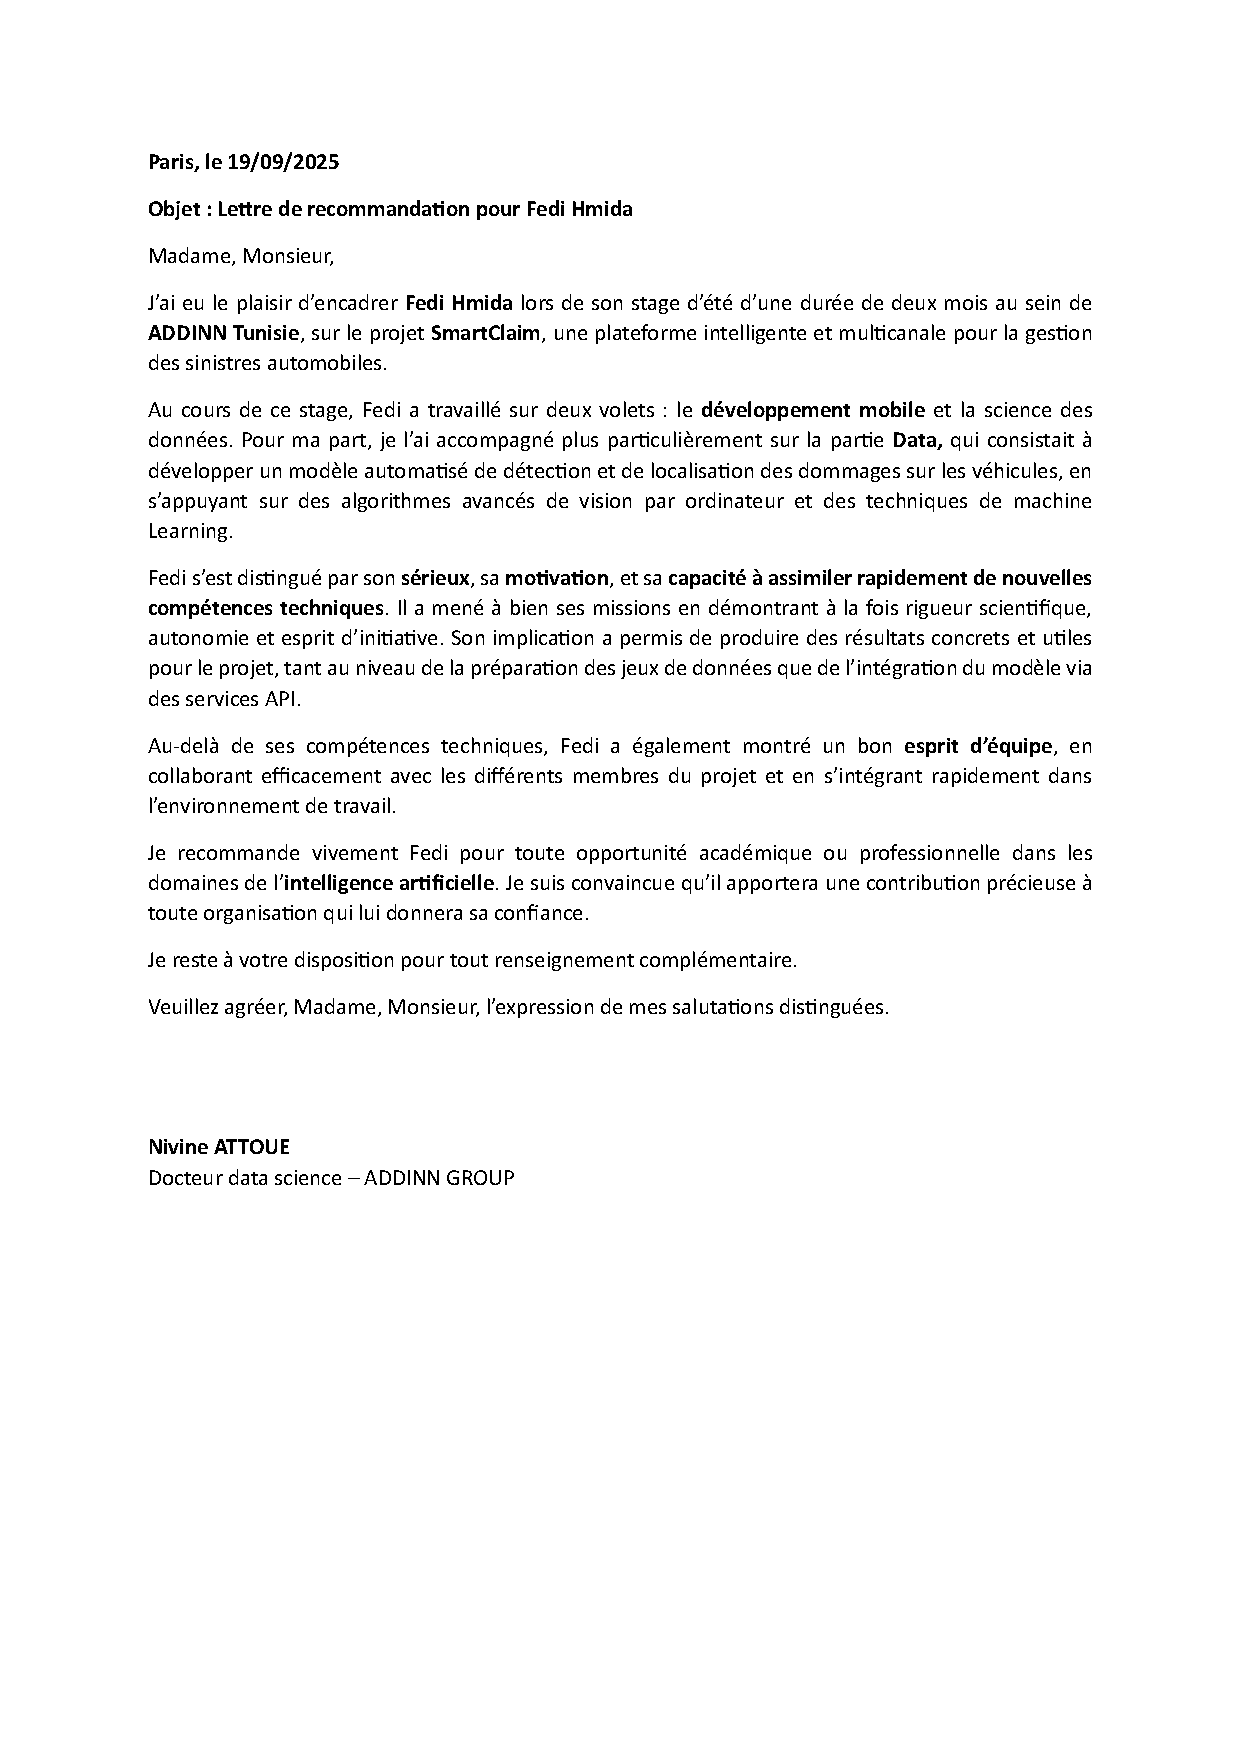
\includegraphics[width=1\textwidth]{Recommendation_FediHmida.pdf}
    \caption{Lettre de recommandation du superviseur Data Science}
    \label{fig:recommendation_data}
\end{figure}

\subsection{Lettre de recommandation - Superviseur Mobile}

\begin{figure}[H]
    \centering
    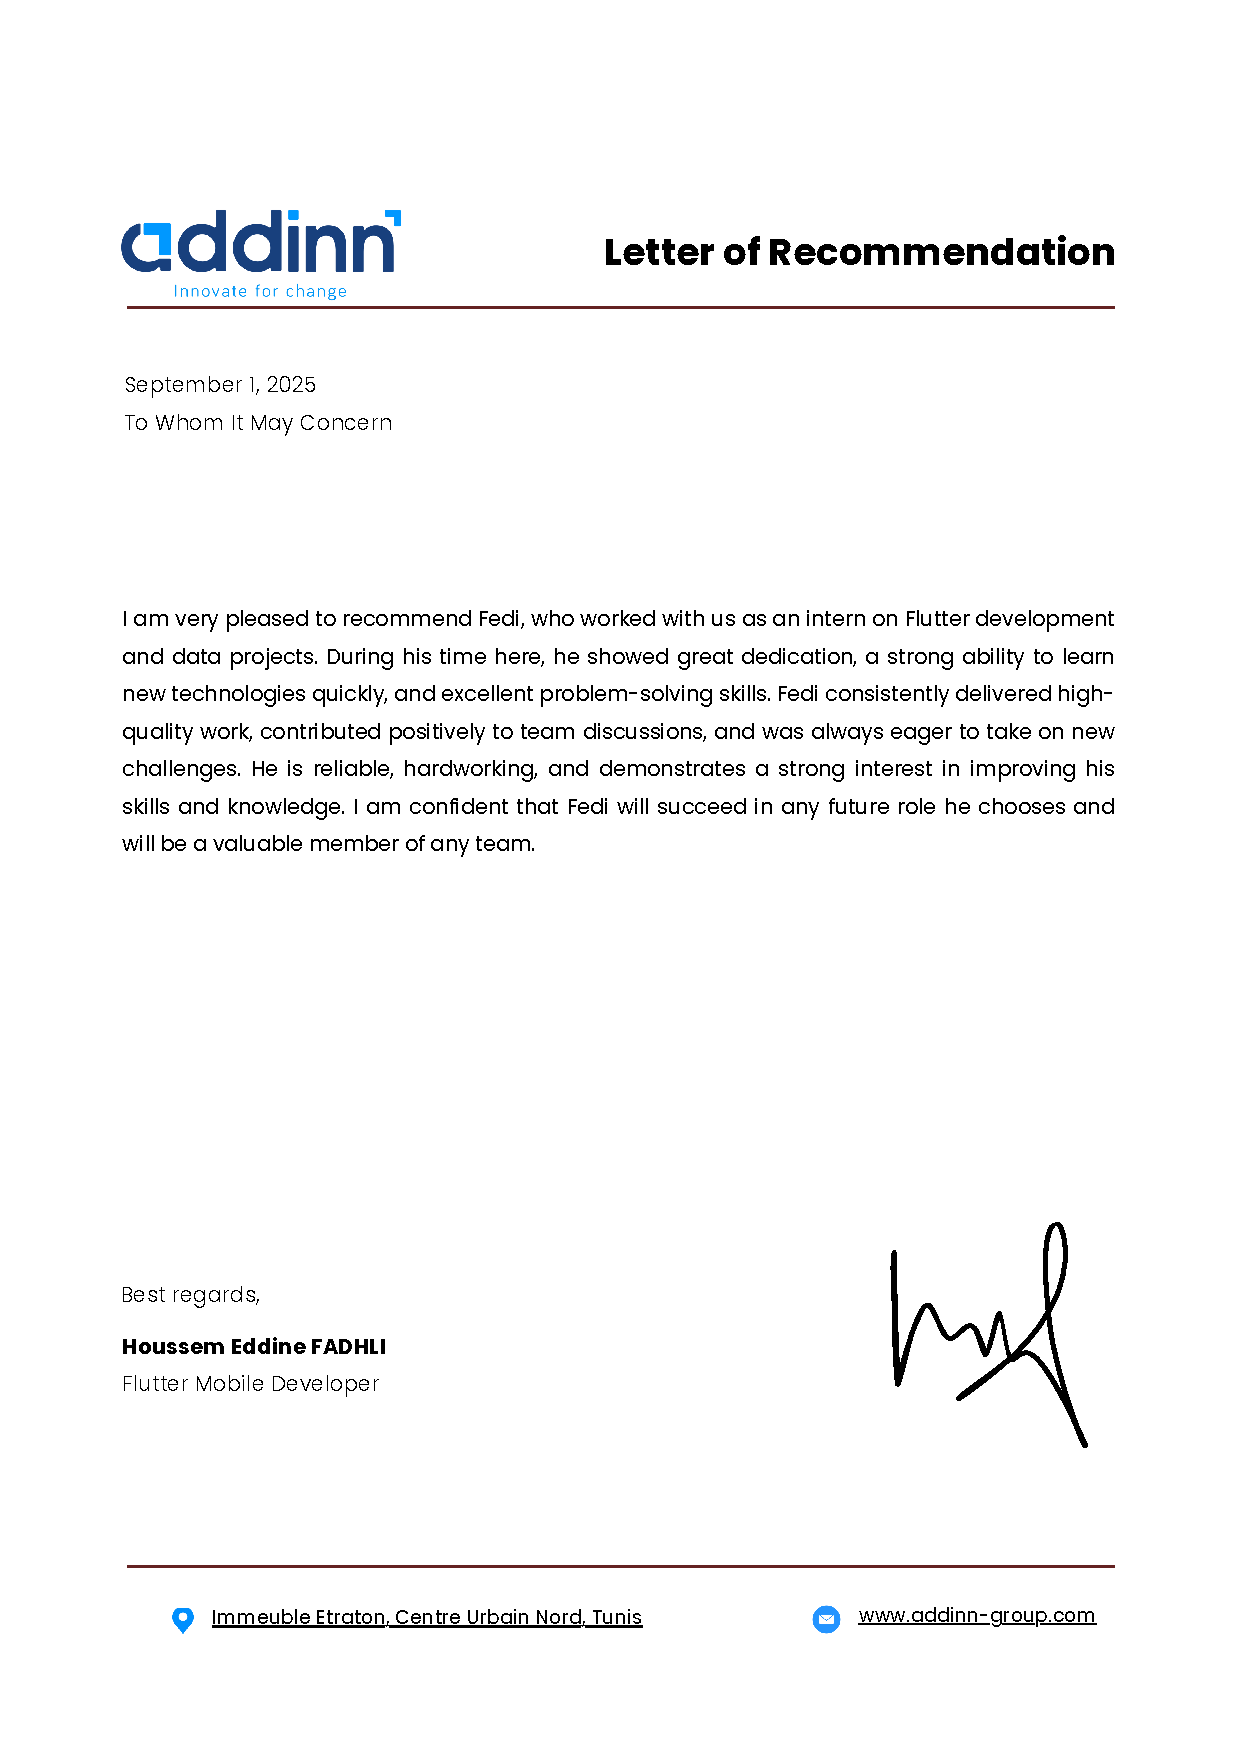
\includegraphics[width=1\textwidth]{Fedi_Hmida_Letter of Recommendation.pdf}
    \caption{Lettre de recommandation du superviseur Mobile}
    \label{fig:recommendation_mobile}
\end{figure}

\textbf{Autres recommandations disponibles de :}
\begin{itemize}
    \item Encadrants de stage (MSign et Addinn Group)
    \item Professeurs ISI Mahdia (formation en licence)
    \item Responsables IEEE ESPRIT Student Branch
\end{itemize}

\textit{Note : D'autres lettres de recommandation sont disponibles sur demande et seront fournies selon les exigences spécifiques du programme IMT Mines Albi.}



% Conclusion
\chapter{Conclusion}

\section{Synthèse de la motivation}

En conclusion de ce dossier, je réaffirme ma forte motivation pour intégrer le programme de mobilité bi-diplômante avec l'IMT Mines Albi. Mon parcours académique solide, mes certifications techniques et linguistiques, ainsi que mes expériences pratiques témoignent de ma préparation à relever les défis de cette formation internationale.

Cette opportunité représente pour moi un tremplin vers une carrière d'ingénieur international, capable d'évoluer dans des environnements multiculturels et de contribuer à des projets d'envergure mondiale.

\section{Engagement et disponibilité}

Je m'engage à :
\begin{itemize}
    \item Maintenir un niveau académique d'excellence durant toute la durée du programme
    \item Respecter les valeurs et règlements des deux institutions
    \item Contribuer positivement à la communauté étudiante internationale
    \item Représenter dignement l'École Esprit au sein de l'IMT Mines Albi
\end{itemize}

Je reste à votre disposition pour tout complément d'information ou entretien que vous jugeriez nécessaire.

\vspace{2cm}

\begin{flushright}
\candidatename\\
\candidateemail\\
\submissiondate
\end{flushright}

\end{document}